
%(BEGIN_QUESTION)
% Copyright 2011, Tony R. Kuphaldt, released under the Creative Commons Attribution License (v 1.0)
% This means you may do almost anything with this work of mine, so long as you give me proper credit

Read and outline the ``Overpressure Protection Devices'' section of the ``Process Safety and Instrumentation'' chapter in your {\it Lessons In Industrial Instrumentation} textbook.  Note the page numbers where important illustrations, photographs, equations, tables, and other relevant details are found.  Prepare to thoughtfully discuss with your instructor and classmates the concepts and examples explored in this reading.

\vskip 10pt

In addition to reading about overpressure protection devices, locate the pressure relief valve on your home's hot-water tank to see a practical example of one.  (Even if you live in an apartment rather than a house, you should have a hot water heater located somewhere where you can inspect it.)  Take a digital photograph of the pressure relief valve, noting its construction and manual test lever.  Why do you think every hot water heater in America is equipped with a pressure relief valve?  Can you see a lift pressure rating documented on this valve?

If you cannot locate your home's hot water heater, open the hood of your car and locate the {\it radiator cap}, which also functions as a pressure relief valve.  Take a digital photograph of the radiator cap, being sure to include the relief tube (where the cap vents excess pressure) in the picture.  Can you see a lift pressure rating documented on this safety device?

\vskip 20pt \vbox{\hrule \hbox{\strut \vrule{} {\bf Suggestions for Socratic discussion} \vrule} \hrule}

\begin{itemize}
\item{} How much pressure does your car's radiator cap lift at?  How high of a water temperature does this correlate to?  Hint: consult a {\it saturated steam table} to determine the steam pressure of boiling water at a given temperature.
\end{itemize}

\underbar{file i02986}
%(END_QUESTION)





%(BEGIN_ANSWER)


%(END_ANSWER)





%(BEGIN_NOTES)

Overpressure protection devices work to protect process piping and vessels from excessive pressure/vacuum.  Rupture disks act like fuses, while relief valves act like self-resetting circuit breakers.  Overpressure events often caused by pipe blockages (e.g. shut block valves) and fires (rise in pressure caused by rise in fluid temperature).

\vskip 10pt

Rupture disks are thin metal structures (usually just a thousandths of an inch in thickness).  Metal disks' burst ratings vary with temperature.  Graphite rupture disks have better corrosion properties and more stable burst pressures, but they tend to fragment rather than tear like metal.

\vskip 10pt

Pressure Relief Valves (PRVs) open proportionately with fluid pressure.  Used on liquid service applications.

\vskip 10pt

Pressure Safety Valves (PSVs) open with ``snap-action'' (deadband).  The deadband (difference) between lifting pressure and re-seating pressure is called the PSV's ``blowdown'' pressure.  PSV's are used on gas/vapor service applications.  This snap action is achieved by designing the valve in such a way that the plug's effective area increases once open.  Some PSV's have an adjustable ``blowdown ring'' for calibrating the amount of snap action desired.

\vskip 10pt

Typically, force exerted on the plug of a PRV or PSV is the actuating stimulus ($F = PA$).  The PRV/PSV serves as its own actuator.

\vskip 10pt

Continuously venting tanks is generally not practical due to fugitive emissions.  This is why safety valves such as the pressure/vacuum Groth design are popular: they normally seal the tank, only lifting when necessary.

\vskip 10pt

Rupture disks and PRVs/PSVs sometimes used in series to minimize corrosion on the valve and reduce fugitive emissions during regular operation.

\vskip 10pt

Some relief valves are equipped with {\it pilot} mechanisms setting the lift and re-seat pressures, the pilot sending actuating fluid pressure to the relief valve rather than the valve itself acting as the trip-setting device.

\vskip 10pt










\vskip 20pt \vbox{\hrule \hbox{\strut \vrule{} {\bf Suggestions for Socratic discussion} \vrule} \hrule}

\begin{itemize}
\item{} How does the action of a rupture disk differ from that of a PSV or PRV?
\item{} Explain why rupture disk pressure ratings are specified at certain temperatures.
\item{} Explain why some rupture disks are manufactured from graphite rather than metal.
\item{} What is the difference between a PSV and a PRV?  What process applications would utilize each one of these valve types?
\item{} Examine the cut-away photograph of the Nupro relief valve, identify its components, and explain how it works.
\item{} Is the Nupro valve shown in the cut-away photograph a PSV or a PRV?  How can we tell?
\item{} The Nupro relief valve shown in the book has a pressure range expressed in units of kPa (340 to 2400 kPa).  Convert this range into PSI (49.3 to 348.1 PSI).
\item{} Explain how to change the lift pressure of a Groth tank overpressure valve.
\item{} Is the Groth valve shown in book a PSV or a PRV?  How can we tell?
\item{} What is a {\it huddling chamber}?
\item{} Why might a safety engineer choose to place a rupture disk downstream of a PRV or PSV?
\item{} Explain the function of a {\it pilot} in an overpressure valve.
\item{} Identify any advantages to using a pilot to actuate an overpressure valve instead of using a self-actuated overpressure valve.
\end{itemize}













\filbreak

Here is the radiator cap on my 1999 Dodge diesel truck, with a 15 PSI lift pressure:

$$\epsfysize=3.5in \includegraphics[width=15.5cm]{i02986x01.eps}$$

15 PSI gauge is 29.7 PSI absolute, which corresponds to approximately 250 degrees Fahrenheit.

%INDEX% Reading assignment: Lessons In Industrial Instrumentation, overpressure protection devices

%(END_NOTES)


